\documentclass[tikz,border=2]{standalone}
\usetikzlibrary{shadows,arrows,shapes,positioning,calc,backgrounds,fit}
\newcommand{\vanish}[1]{}
\usepackage{colortbl}
\usepackage{array}
\usepackage{amssymb}
\usepackage{multirow}
\newcommand{\shaded}[1]{\cellcolor{black!20}{#1}}
\newcommand{\calc}[1]{\mbox{$\mathcal{C}_{#1}$}}
\pdfpageattr {/Group << /S /Transparency /I true /CS /DeviceRGB>>}
\newcommand{\mathtttt}{}
% Define the layers to draw the diagram
%
\begin{document}
%% \pgfdeclarelayer{bg}
%% \pgfdeclarelayer{fg}
%% \pgfsetlayers{bg,main,fg}
%
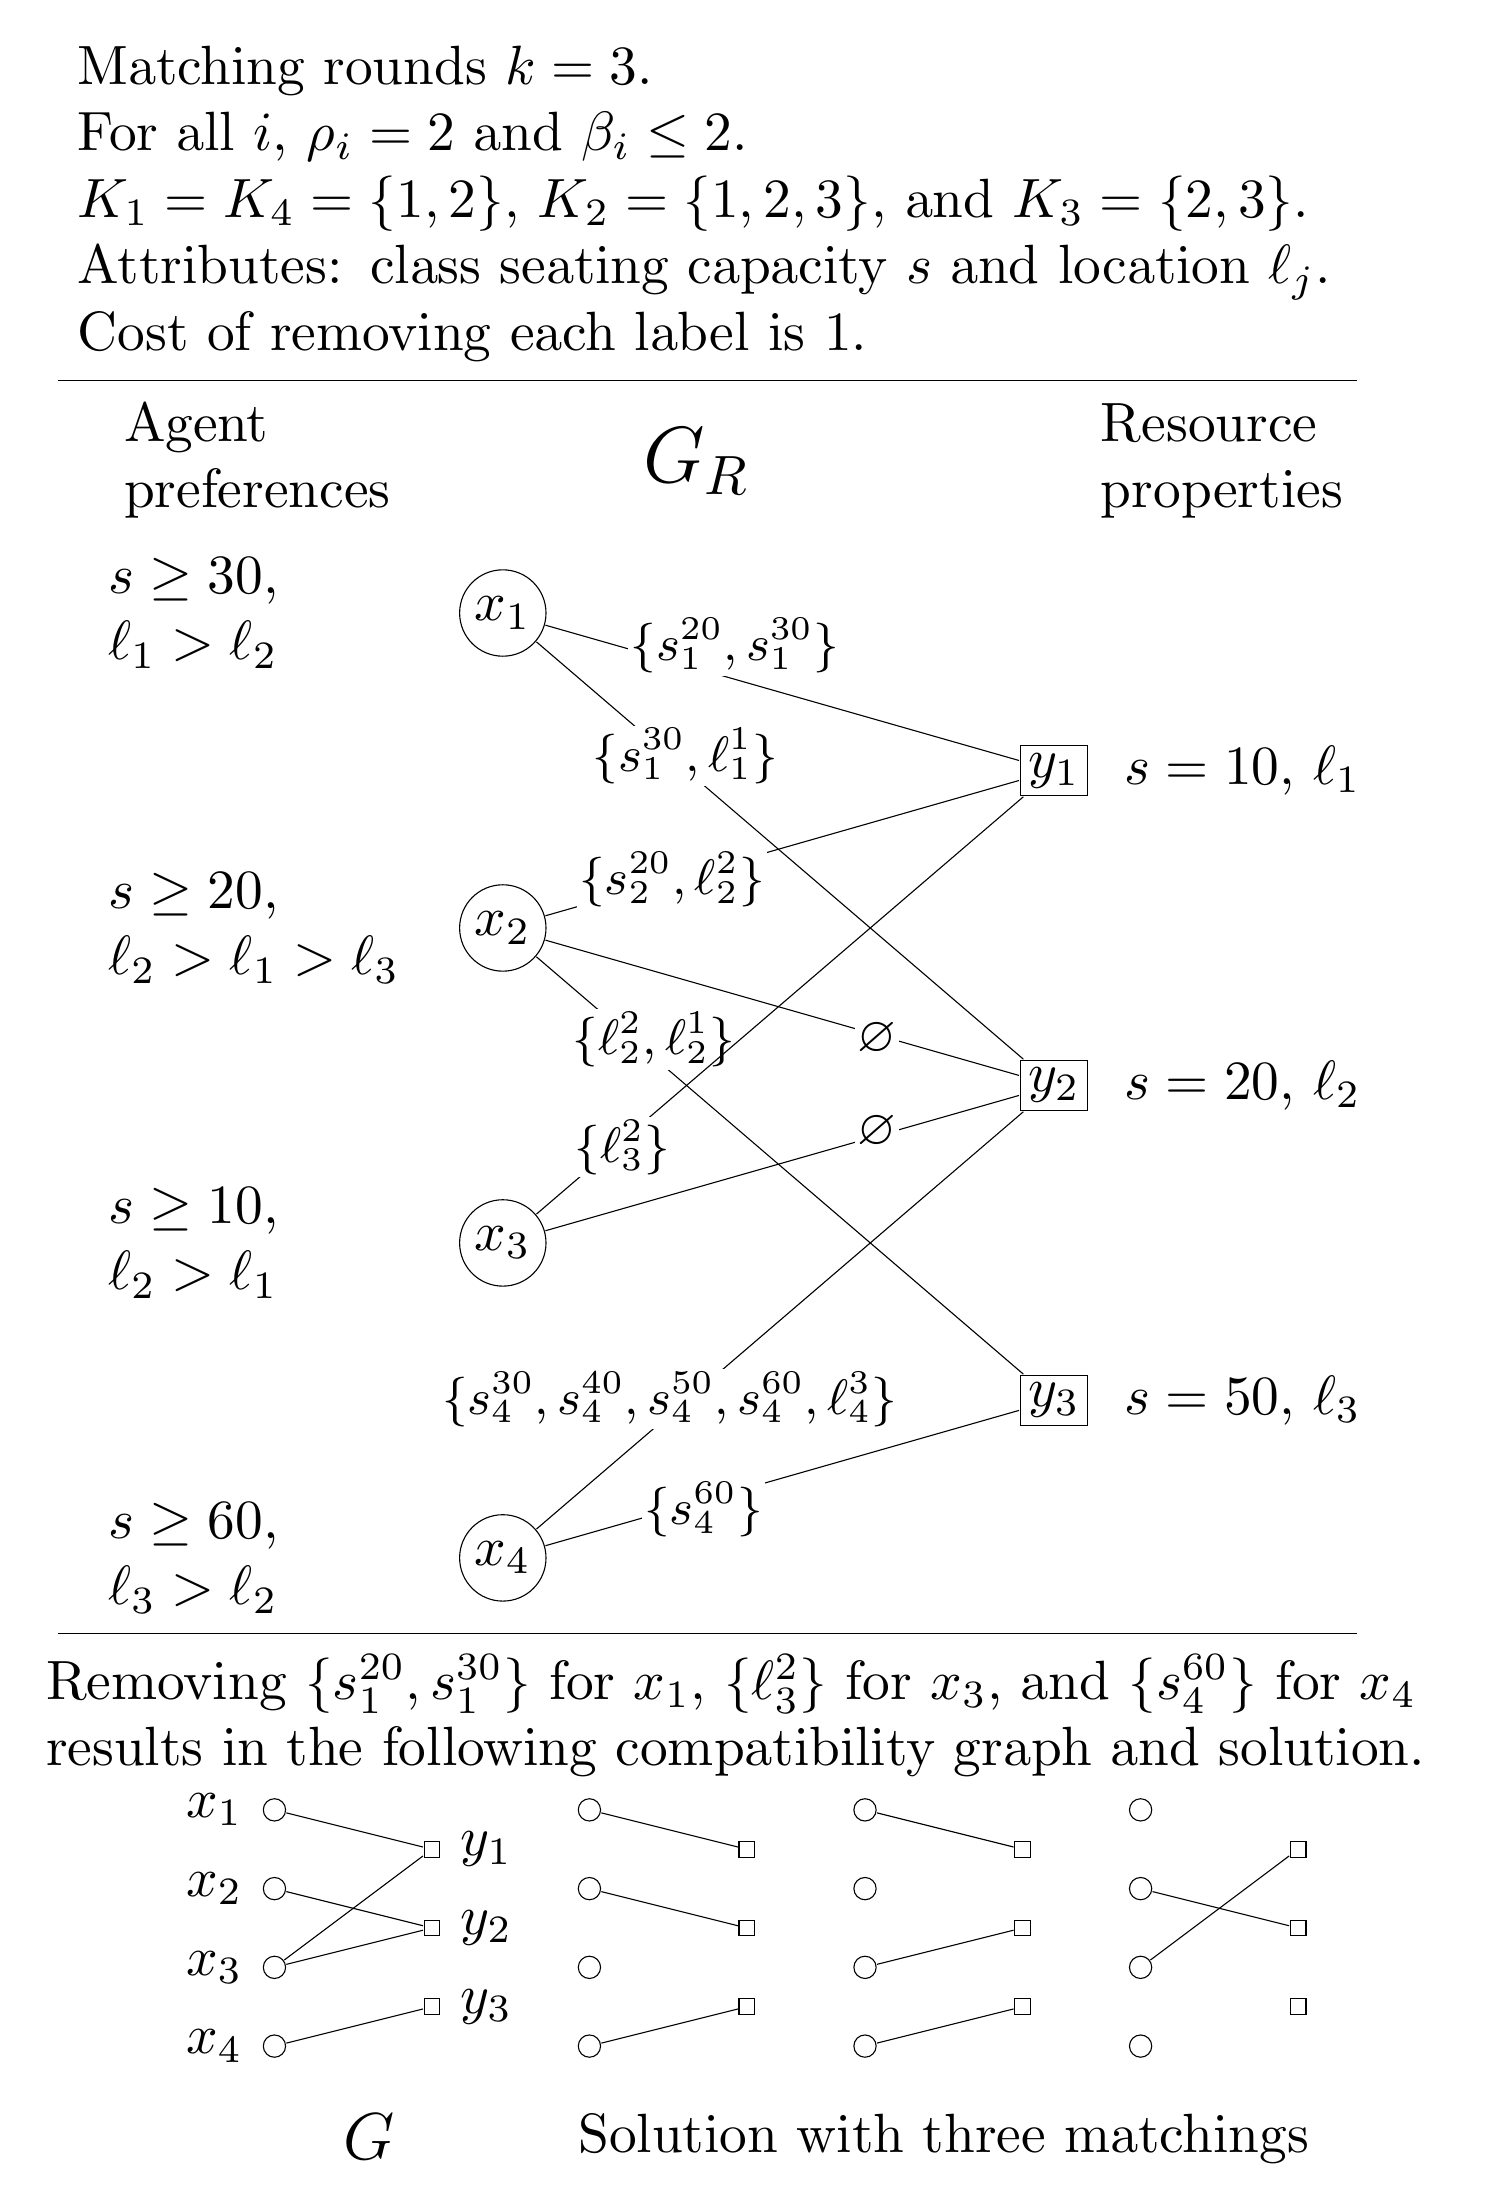
\begin{tikzpicture}
[scale=2,node distance=.5cm, transform shape,
    agent/.style={draw,shape=circle,inner sep=.5mm},
    res/.style={shape=rectangle,draw,inner sep=.5mm},
    lab/.style={fill=white,font=\small,inner sep=.5pt},
    prop/.style={text width=2cm},
myedge/.style={>=latex', shorten >=.0pt, shorten <=.0pt,semithick}]
%%%%%%%%%%
%%%%% The underlying graph with preferences and properties
\begin{scope}
    \node[text width=8cm] (desc) {Matching rounds~$k=3$. \\
        For all~$i$, $\rho_i=2$ and $\beta_i\le2$. \\
        $K_1=K_4=\{1,2\}$, $K_2=\{1,2,3\}$, and $K_3=\{2,3\}$.\\
        Attributes: class seating capacity~$s$ and location~$\ell_j$.\\
    Cost of removing each label is $1$.
};
    \draw (desc.south west) -- (desc.south east);
\end{scope}
%%
\begin{scope}[shift={(-1.3,-2.6)}]
%% nodes
\node (x1) [agent] at (0,0)  {$x_1$};
\node (x2) [agent] at (0,-2) {$x_2$};
\node (x3) [agent] at (0,-4) {$x_3$};
\node (x4) [agent] at (0,-6) {$x_4$};
\node (y1) [res] at (3.5,-1) {$y_1$};
\node (y2) [res] at (3.5,-3) {$y_2$};
\node (y3) [res] at (3.5,-5) {$y_3$};
%% agent preferences
\node (px1) [prop,left=of x1,shift={(.4,0)}] {$s\ge30$, \\$\ell_1>\ell_2$};
\node (px2) [prop,left=of x2,shift={(.4,0)}] {$s\ge20$, \\$\ell_2>\ell_1>\ell_3$};
\node (px3) [prop,left=of x3,shift={(.4,0)}] {$s\ge10$, \\$\ell_2>\ell_1$};
\node (px4) [prop,left=of x4,shift={(.4,0)}] {$s\ge60$, \\$\ell_3>\ell_2$};
\node (tap) [above=of px1, text width=1.8cm, shift={(0,-.5)}] {Agent \\preferences};
\node (Gr) [right=of tap,shift={(.75,0)}] {\Large $G_R$};
%% resource properties
\node (py1) [right=of y1,shift={(-.4,0)}] {$s=10$, $\ell_1$};
\node (py2) [right=of y2,shift={(-.4,0)}] {$s=20$, $\ell_2$};
\node (py3) [right=of y3,shift={(-.4,0)}] {$s=50$, $\ell_3$};
\node (trp) [text width=1.8cm] at (py1|-tap) {Resource \\properties};
%% edges
\draw (x1) -- node[lab,shift={(-.3,.3)}]{$\{\mathtttt{s_1^{20}},\mathtttt{s_1^{30}}\}$} (y1); 
\draw (x1) -- node[lab,shift={(-.6,.6)}]{$\{\mathtttt{s_1^{30}},\mathtttt{\ell_1^{1}}\}$} (y2); 
\draw (x2) -- node[lab,shift={(-.7,-.2)}]{$\{\mathtttt{s_2^{20}},\mathtttt{\ell_2^{2}}\}$} (y1); 
\draw (x2) -- node[lab,shift={(.6,-.2)}]{$\varnothing$} (y2); 
\draw (x2) -- node[lab,shift={(-.8,.8)}]{$\{\mathtttt{\ell_2^{2}},\mathtttt{\ell_2^{1}}\}$} (y3); 
\draw (x3) -- node[lab,shift={(-1,.-.9)}]{$\{\mathtttt{\ell_3^{2}}\}$} (y1); 
\draw (x3) -- node[lab,shift={(.6,.2)}]{$\varnothing$} (y2); 
\draw (x4) --
node[lab,shift={(-.7,.-.5)}]{$\{\mathtttt{s_4^{30}},\mathtttt{s_4^{40}},\mathtttt{s_4^{50}},\mathtttt{s_4^{60}},\mathtttt{\ell_4^{3}}\}$} (y2); 
\draw (x4) --
node[lab,shift={(-.5,.-.2)}]{$\{\mathtttt{s_4^{60}}\}$} (y3); 
\node (anc) at ($(x4.south)+(0,-.2)$) {};
\draw (desc.south west|-anc) -- (desc.south east|-anc);
\end{scope}
%%
\begin{scope}[shift={(.3,-9.6)}]
    \node [text width=9cm] {Removing
$\{\mathtttt{s_1^{20}},\mathtttt{s_1^{30}}\}$ for $x_1$,
 $\{\mathtttt{\ell_3^{2}}\}$ for
$x_3$, and $\{\mathtttt{s_4^{60}}\}$ for
$x_4$ results in the following compatibility graph and solution.};
\end{scope}
%% Gc
\begin{scope}[shift={(-2.75,-10.2)},local bounding box=Gc]
\node (x1) [agent, label=left:$x_1$] at (0,0)  {};
\node (x2) [agent, label=left:$x_2$] at (0,-.5) {};
\node (x3) [agent, label=left:$x_3$] at (0,-1) {};
\node (x4) [agent, label=left:$x_4$] at (0,-1.5) {};
\node (y1) [res, label=right:$y_1$] at (1,-.25) {};
\node (y2) [res, label=right:$y_2$] at (1,-.75) {};
\node (y3) [res, label=right:$y_3$] at (1,-1.25) {};
\draw (x1) -- (y1);
\draw (x2) -- (y2);
\draw (x3) -- (y1);
\draw (x3) -- (y2);
\draw (x4) -- (y3);
\node [below=of y3,shift={(-.4,0)}] {\large$G$};
%%\draw (1.5,.1) -- +(0,-1.7);
\end{scope}
%% matching 1
\begin{scope}[shift={(-.75,-10.2)}]
\node (x1) [agent] at (0,0)  {};
\node (x2) [agent] at (0,-.5) {};
\node (x3) [agent] at (0,-1) {};
\node (x4) [agent] at (0,-1.5) {};
\node (y1) [res] at (1,-.25) {};
\node (y2) [res] at (1,-.75) {};
\node (y3) [res] at (1,-1.25) {};
\draw (x1) -- (y1);
\draw (x2) -- (y2);
\draw (x4) -- (y3);
\end{scope}
%% matching 2
\begin{scope}[shift={(1,-10.2)}]
\node (x1) [agent] at (0,0)  {};
\node (x2) [agent] at (0,-.5) {};
\node (x3) [agent] at (0,-1) {};
\node (x4) [agent] at (0,-1.5) {};
\node (y1) [res] at (1,-.25) {};
\node (y2) [res] at (1,-.75) {};
\node (y3) [res] at (1,-1.25) {};
\draw (x1) -- (y1);
\draw (x3) -- (y2);
\draw (x4) -- (y3);
\node [below=of y3,shift={(-.5,0)}] {Solution with three matchings};
\end{scope}
%% matching 3
\begin{scope}[shift={(2.75,-10.2)}]
\node (x1) [agent] at (0,0)  {};
\node (x2) [agent] at (0,-.5) {};
\node (x3) [agent] at (0,-1) {};
\node (x4) [agent] at (0,-1.5) {};
\node (y1) [res] at (1,-.25) {};
\node (y2) [res] at (1,-.75) {};
\node (y3) [res] at (1,-1.25) {};
\draw (x2) -- (y2);
\draw (x3) -- (y1);
\end{scope}
\end{tikzpicture}
\end{document}
